\documentclass[12pt]{article}
\usepackage{../../../tex/universal}
\input{../../../tex/ambry_commands}
\begin{document}
\author{Jakub Ambroz}
\begin{center}
    \begin{Huge}
    RPH Spam filter
    \end{Huge}\\
    \vspace{2mm}
    \begin{Large}Jakub Ambroz a Kateřina Kučerová\end{Large}\\
    \vspace{2mm}
    \today
\end{center}
\section{Úvod}
Cílem naší práce bylo zhotovit jednoduchý spam filter. Celé zadání na \url{https://cw.fel.cvut.cz/wiki/courses/b4b33rph/cviceni/spam/start}.\\
Hlavní přínosem pro nás jako studenty jsou zejména nově nabyté zkušenosti v oblasti objektově orientovaného programování, práce v týmu či dokonce základy strojového učení. 
\section{Popis filtru}
\subsection{Předzpracování dat}
Pomocí knihovny emails, jsme vytáhli ze souboru jak obsah mailu, tak i metadata o něm. Obsah pomocí "str.replace" a \emph{regular expression} jsme pročistili mail od html tagů (ikdyž ne úplně úspěšně, protože jedno z nejčastějších spamových slov bylo '=2'), rozdělili na jednotlivá slova se shodnou kapitalizací. Dále jsme pak pracovali s polem slov.
\subsection{Učení}
Náš filtr funguje na principu počítání četnosti výskytu slov ve spamech a v hamech. Po spočtení všech četností procházíme testovaný mail slovo po slovu. Pokud se nachází častěji ve spamu (tj. četnost ve spam mailech děleno počtem slov ve spam mailech je vyšší), zvětšujeme „spamovou“ proměnnou o jedna, pokud je častěji v hamech, zvyšujeme naopak „hamovou“ proměnnou. Pokdu dojde ke shodě (tedy i 0==0), pokračujeme k dalšímu slovu.\\
Poté porovnáváme proměnné pro daný e-mail a tím určujeme, zdali se jedná o spam či nikoliv.\\
Následoval upgrade, kde počítáme četnosti hodnot jednotlivých metadat (ty ani nijak neupravujeme) o e-mailu. To mělo občas lepší a občas horší výsledky než využívaní slov. A nejlepších výsledků jsme dosáhli, když jsme obě tyto metody klasifikace spojili logickým ano. Důvodem je zřejmě to, že jsme odstranili zejména false positive, které jsou pro kvalitu horší než false negatives.
\subsection{Datová sada}
K testování jsme udělali script, částečně v Pythonu a částečně v shellu, který náhodně rozdělil dodaná data na trénovací a testovací sadu v určitém poměru. Tím jsme otestovali, že se nám nepodařilo overfitovat.
\subsection{Kvalita}
Pohybovala se stabilně přes $0.8$ a občas i přes $0.9$. V turnaji to bylo $0.85, 0.72, 0.82$.
\begin{figure}[htp]
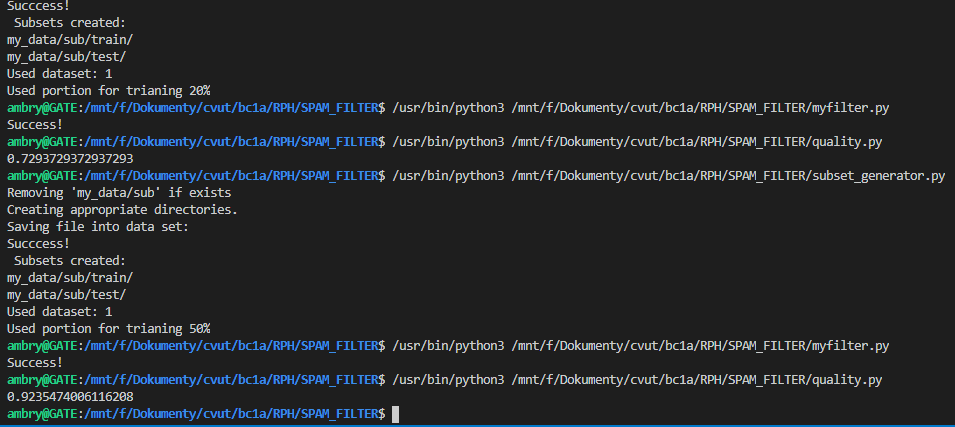
\includegraphics[width=1\textwidth]{uspesnost.png}
\end{figure}
\section{Spolupráce v týmu}
Pro práci ve skupině nám posloužil GitLab (viz \url{https://gitlab.fel.cvut.cz/ambrojak/rph-spam-filter, pokud bude zveřejněno}). Ten byl ale použit převážně jen k verzování (a vytvoření todo listu pomocí issues). K spolupráci na kódu posloužil spíše Liveshare extension ve VSCode.\\
Díky němu jsme mohli pracovat na kódu zároveň. Další výhodou bylo, že v něm šlo sdílet i příkazovou řádku z WSL (Windows Subsystem for Linux), takže kód mohl spouštět i vzdáleně připojený. Ten navíc nemusí nic nastavovat (např. \LaTeX je relativně složité nastavit a zprovoznit) a může využít již nastavené funkční prostředí hosta.
\section{Závěr a zhodnocení}
K dalšímu zlepšení - v úvahu připadá třeba využití počtu odkazů, či vykřičníků. Eventuálně by bylo vhodné upravit spíše na opravdovou Bayesovskou klasifikaci. To by znamenalo předělat většinu kódu - nastala tedy chyba plánování. Další možným vylepšením by byla například určitá tokenizace metadat, kvalita tohoto filtru se ale ukázala být dostačující.\\
Na závěr bychom chtěli poznamenat, že nás vypracovávání úlohy velmi bavilo. Napadá nás, že kdybychom měli více času, zkusili bychom i něco komplikovanějšího.
\section{Zdroje}
"Já jsem jenom počítal kolikrát je tam to slovo a ono to mělo dobrý výsledky" - Jakub Kraus
\end{document}